\documentclass[11pt,a4paper]{article}

\usepackage[utf8]{inputenc}
\usepackage[T1]{fontenc}
\usepackage{amsmath}
\usepackage{graphicx}
\usepackage{hyperref}
\usepackage{listings}
\usepackage{xcolor}
\usepackage{booktabs}
\usepackage{float}
\usepackage{algorithm}
\usepackage{algpseudocode}
\usepackage{tcolorbox}
\usepackage{fancyhdr}
\usepackage{geometry}
\usepackage{titlesec}
\usepackage{enumitem}

% Page geometry
\geometry{
    top=2.5cm,
    bottom=2.5cm,
    left=2.5cm,
    right=2.5cm
}

% Custom colors
\definecolor{primaryblue}{RGB}{41, 128, 185}
\definecolor{secondaryblue}{RGB}{52, 152, 219}
\definecolor{codebackground}{RGB}{250, 250, 250}
\definecolor{codecomment}{RGB}{102, 153, 102}
\definecolor{codekeyword}{RGB}{0, 119, 170}
\definecolor{codestring}{RGB}{170, 51, 119}

% Section styling
\titleformat{\section}
    {\color{primaryblue}\Large\bfseries}
    {\thesection}{1em}{}
\titleformat{\subsection}
    {\color{secondaryblue}\large\bfseries}
    {\thesubsection}{1em}{}

% Code listing style
\lstdefinestyle{pythonstyle}{
    backgroundcolor=\color{codebackground},
    commentstyle=\color{codecomment},
    keywordstyle=\color{codekeyword}\bfseries,
    stringstyle=\color{codestring},
    basicstyle=\ttfamily\footnotesize,
    breakatwhitespace=false,
    breaklines=true,
    captionpos=b,
    keepspaces=true,
    numbers=left,
    numbersep=5pt,
    showspaces=false,
    showstringspaces=false,
    showtabs=false,
    tabsize=2,
    frame=single,
    rulecolor=\color{black!30},
    language=Python
}
\lstset{style=pythonstyle}

% Custom box styles
\newtcolorbox{infobox}[1][]{
    colback=blue!5,
    colframe=blue!75!black,
    fonttitle=\bfseries,
    title=#1
}

\newtcolorbox{resultbox}[1][]{
    colback=green!5,
    colframe=green!75!black,
    fonttitle=\bfseries,
    title=#1
}

% Header and footer
\pagestyle{fancy}
\fancyhf{}
\fancyhead[L]{\textit{Temperature detection from cloud cover}}
\fancyhead[R]{\thepage}
\renewcommand{\headrulewidth}{0.4pt}

\title{
    \textcolor{primaryblue}{\textbf{\LARGE Temperature detection from cloud cover}}\\
    \vspace{0.5cm}
    \Large Phase 2: Cloud Coverage Detection
}
\author{CLOUD COVER: Ayush Kumar Mishra, Akshat Kumar , Aditya Prakash}
\date{\today}

\begin{document}

\maketitle

\begin{abstract}
[Project Overview]:\\

This document presents Phase 2 of our comprehensive weather prediction system, focusing on cloud coverage detection using deep learning and computer vision techniques. The system implements a hybrid approach combining CLIP-based feature extraction with CatBoost regression, achieving robust performance in cloud coverage estimation. This phase lays the groundwork for Phase 3, which will implement temperature prediction based on cloud coverage patterns.

\end{abstract}

\tableofcontents
\newpage

\section{Introduction}
\subsection{Project Context}
This project represents Phase 2 of a three-phase implementation:
\begin{enumerate}[label=\textcolor{primaryblue}{Phase \arabic*:}]
    \item SOP Submission
    \item \textbf{Cloud Coverage Detection} (Current Phase)
    \item Temperature Prediction from Cloud Coverage prediction , we are getting from phase-2 code (Upcoming)
\end{enumerate}

\subsection{Problem Statement}
Cloud coverage prediction serves as a crucial intermediate step in our temperature prediction system. This phase focuses on developing accurate cloud coverage estimation using ground-based sky cameras and deep learning techniques.


\section{Technical Implementation}
\subsection{Model Architecture}

\subsubsection{CLIP-Based Feature Extraction}
\begin{lstlisting}
class MemoryEfficientImageEncoder(nn.Module):
    def __init__(self, cfg):
        super().__init__()
        self.model = timm.create_model(
            cfg.model_name,
            pretrained=cfg.pretrained,
            num_classes=0,
            global_pool='avg'
        )
\end{lstlisting}

% Space for web interface screenshot
\begin{figure}[H]
\centering
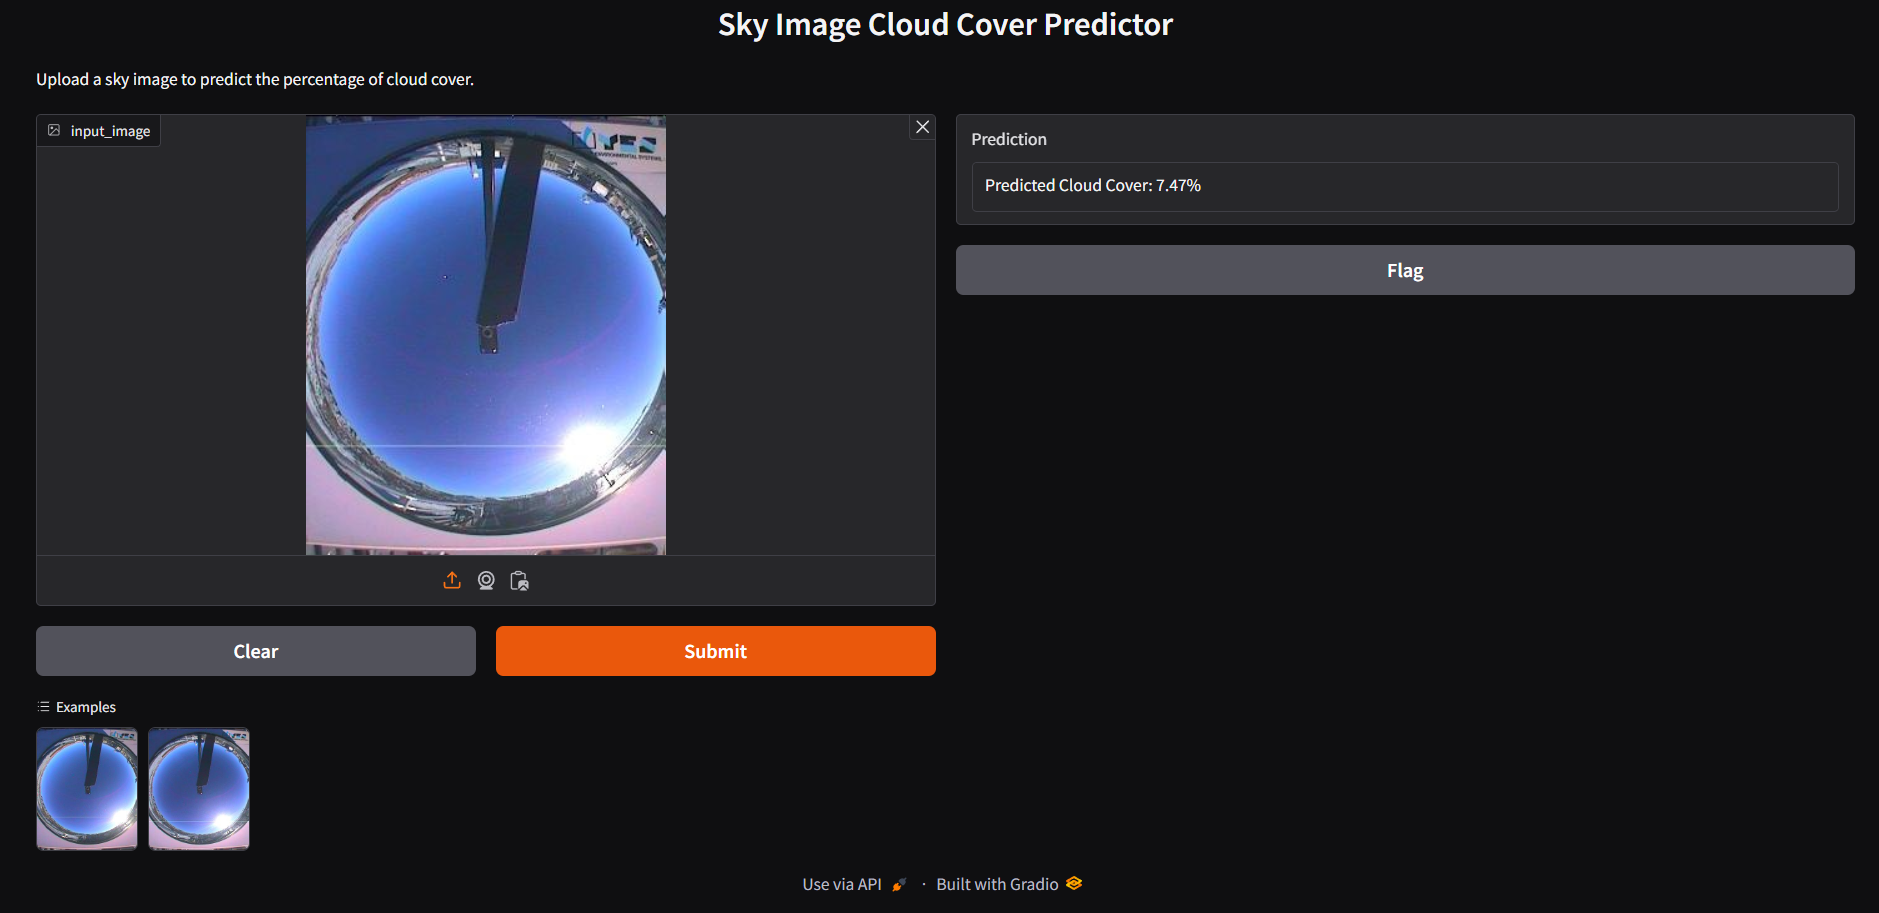
\includegraphics[width=0.9\textwidth]{website.png}
\caption{Web Interface for Cloud Coverage Prediction}
\label{fig:interface}
\end{figure}

\section{Performance Metrics}
\begin{resultbox}[Model Performance Results]
\begin{verbatim}
Train Metrics:
    MAE: 3.06
    RMSE: 4.52
    R2: 0.975

Validation Metrics:
    MAE: 5.80
    RMSE: 9.62
    R2: 0.888

Test Metrics:
    MAE: 5.81
    RMSE: 9.69
    R2: 0.886
\end{verbatim}
\end{resultbox}



\subsection{Project Objectives}
\begin{itemize}
    \item Develop an accurate cloud coverage prediction system
    \item Implement efficient data preprocessing pipeline
    \item Create memory-optimized model training framework
    \item Deploy an accessible web interface for predictions
\end{itemize}

\section{Dataset}
\subsection{Data Sources}
The project utilizes two main data components:
\begin{itemize}
    \item \texttt{cloud\_data\_cleaned1.csv}: Contains metadata and labels
    \item Sky camera images dataset: Collection of hemispheric sky images
\end{itemize}

\subsection{Dataset Structure}
\begin{table}[H]
\centering
\begin{tabular}{@{}lll@{}}
\toprule
Column & Type & Description \\
\midrule
image\_name & string & Unique identifier for each image \\
label & string & Descriptive cloud coverage label \\
opaque\_clouds & float & Percentage of cloud coverage \\
\bottomrule
\end{tabular}
\caption{Dataset Schema}
\end{table}

\section{Data Preprocessing}
\subsection{Image Conversion Pipeline}
\begin{algorithm}[H]
\caption{Parallel Image Conversion}
\begin{algorithmic}[1]
\State \textbf{Input:} Directory containing RAW images
\State \textbf{Output:} Converted JPEG images
\For{each image in directory}
    \State Create ThreadPoolExecutor
    \State Submit conversion task
    \If{conversion successful}
        \State Remove original RAW file
        \State Log success
    \Else
        \State Log error
    \EndIf
\EndFor
\end{algorithmic}
\end{algorithm}

\subsection{Dataset Cleaning}
The dataset cleaning process involves:
\begin{itemize}
    \item Removing invalid image entries
    \item Standardizing image names
    \item Validating image-label pairs
    \item Handling missing values
\end{itemize}

\section{Model Architecture}
\subsection{CLIP-Based Feature Extraction}

% Space for architecture diagram
\begin{figure}[H]
    \centering
    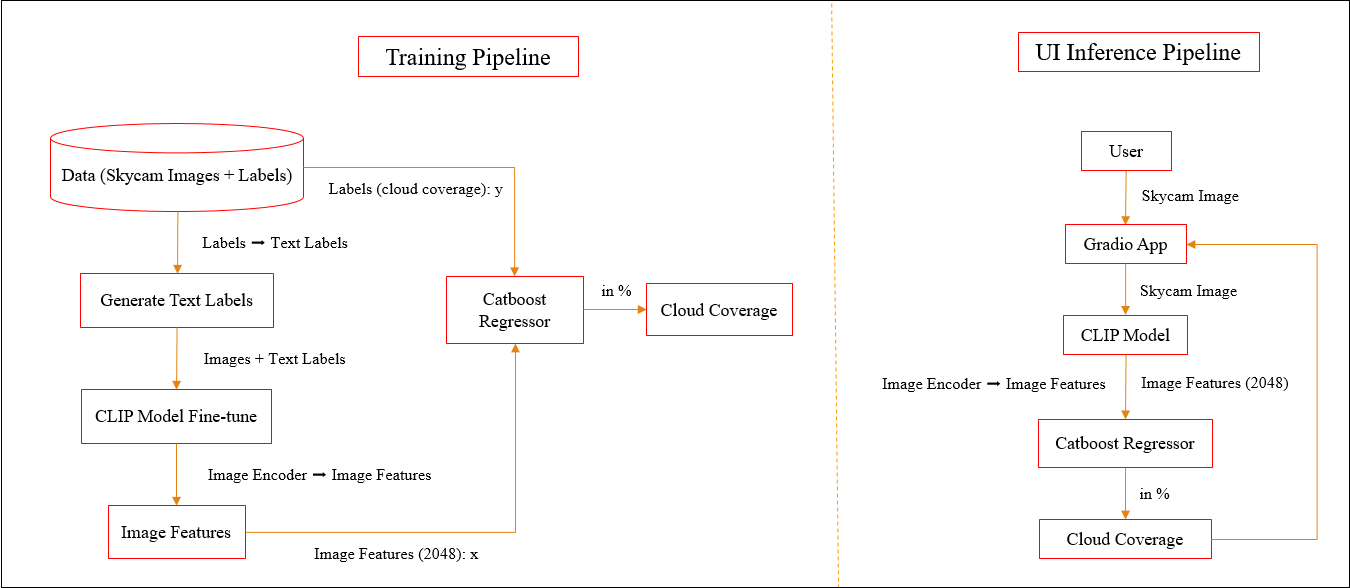
\includegraphics[width=0.8\textwidth]{archi.png}
    \caption{System Architecture Overview}
    \label{fig:architecture}
\end{figure}
    

The model consists of three main components:

\subsubsection{Image Encoder}
\begin{lstlisting}
class MemoryEfficientImageEncoder(nn.Module):
    def __init__(self, cfg):
        super().__init__()
        self.model = timm.create_model(
            cfg.model_name,
            pretrained=cfg.pretrained,
            num_classes=0,
            global_pool='avg'
        )
\end{lstlisting}

\subsubsection{Text Encoder}
\begin{lstlisting}
class MemoryEfficientTextEncoder(nn.Module):
    def __init__(self, cfg):
        super().__init__()
        self.model = DistilBertModel.from_pretrained(
            cfg.text_encoder_model
        )
\end{lstlisting}

\subsubsection{Projection Head}
\begin{lstlisting}
class ProjectionHead(nn.Module):
    def __init__(self, cfg, embedding_dim):
        super().__init__()
        self.projection = nn.Linear(
            embedding_dim, 
            cfg.projection_dim
        )
\end{lstlisting}

\section{Training Pipeline}
\subsection{Memory Optimization Techniques}
\begin{itemize}
    \item Gradient checkpointing
    \item Mixed precision training
    \item Efficient data loading with sharding
    \item Memory usage tracking
\end{itemize}

\subsection{Training Configuration}
\begin{lstlisting}
class Config:
    model_name = 'resnet50'
    image_embedding = 2048
    text_embedding = 768
    projection_dim = 256
    batch_size = 16
    epochs = 15
    temperature = 1.0
\end{lstlisting}

\subsection{Training Process}
\begin{algorithm}[H]
\caption{Training Pipeline}
\begin{algorithmic}[1]
\State Initialize model and optimizer
\State Load and preprocess data
\For{each epoch}
    \State Train model
    \State Validate performance
    \If{best performance}
        \State Save checkpoint
    \EndIf
    \State Update learning rate
\EndFor
\end{algorithmic}
\end{algorithm}

\section{CatBoost Model Training}
\subsection{Feature Engineering}
The CatBoost model uses features extracted from:
\begin{itemize}
    \item CLIP embeddings
    \item Image statistics
    \item Temporal information
\end{itemize}

\subsection{Model Configuration}
\begin{lstlisting}
params = {
    'iterations': 1000,
    'learning_rate': 0.05,
    'depth': 6,
    'loss_function': 'RMSE'
}
\end{lstlisting}

\subsection{Training and Evaluation}
\begin{itemize}
    \item Cross-validation setup
    \item Hyperparameter optimization
    \item Performance metrics monitoring
\end{itemize}

\section{Results and Discussion}
\subsection{Performance Metrics}
\begin{verbatim}
---------------------------------------------------
Train MAE: 3.063867080191343
Train RMSE: 4.519084504196453
Train MSE: 20.422124756068502
Train R2: 0.9753638347539638
---------------------------------------------------
---------------------------------------------------
Valid MAE: 5.798734045374874
Valid RMSE: 9.624912586359335
Valid MSE: 92.63894229505833
Valid R2: 0.8879491192051271
---------------------------------------------------
---------------------------------------------------
Test MAE: 5.812910249786526
Test RMSE: 9.69202086124033
Test MSE: 93.93526837471777
Test R2: 0.886006145423602
---------------------------------------------------

\end{verbatim}

\caption{Model Performance Metrics}
\end{table}



\section{Future Work}
\subsection{Phase 3 Integration}
The cloud coverage percentages obtained in this phase will serve as input features for Phase 3's temperature prediction model. Key integration points include:

\begin{itemize}
    \item Cloud coverage pattern analysis
    \item Temperature correlation modeling
    \item Integration with meteorological data
    \item Enhanced prediction pipeline
\end{itemize}


\section{Conclusion}
Phase 2 successfully establishes a robust cloud coverage detection system, achieving an R² score of 0.886 on the test set. This foundation will be crucial for the temperature prediction implementation in Phase 3.

\bibliographystyle{plain}
\bibliography{references}

\end{document}